\section{Dielektrische Spiegel}
In dem Laserresonator werden, wie oben bereits diskutiert, Spiegel mit hohen Reflektivitäten benötigt. 
Hierfür werden meistens dielektrische oder Bragg Spiegel verwendet. 
Das besondere an diesen Spiegeln ist, dass sie aus unterschiedlichen Schichten mit verschiedenen Brechungsindizies bestehen.
Diese Schichten werden abwechselnd mit hohen und niedrigen Brechungsindex auf eine Glasplatte aufgetragen. 
Die Dicke dieser Schichten ist häufig $d = \frac{\lambda}{2}$ oder $d=\frac{\lambda}{4}$. 
$\lambda$ ist hierbei die Wellenlänge des zu reflektierenden Lichts, d.h. es wird nur ein Teil des Spektrums reflektiert.
Trifft ein Strahl auf den Spiegel so wird ein Teil des Strahls am optisch dickeren Medium mit einem Phasensprung 
um $\pi$ reflektiert und der andere Teil transmittiert. Am optisch dünneren Medium wird dieser Strahl ohne Phasensprung reflektiert. 
Somit hat der Strahl beim Austreten dieselbe Phase, wie der zuerst reflektierte Strahl. Dieser Vorgang ist beliebig oft wiederholbar.
Durch geeignete Wahl von Schichtdicke und der Brechungsindizies kann es zur konstruktiven Interferenz zwischen den reflektierten 
Teilstrahlen kommen. Somit kann man hohe Reflektivitäten nahe 1 erreichen. \citep[vgl.][]{spiegel}\\
Zur Verdeutlichung ist noch eine schematische Darstellung eines dielektrischen Spiegels eingefügt:
\begin{figure}[h]
    \centering
    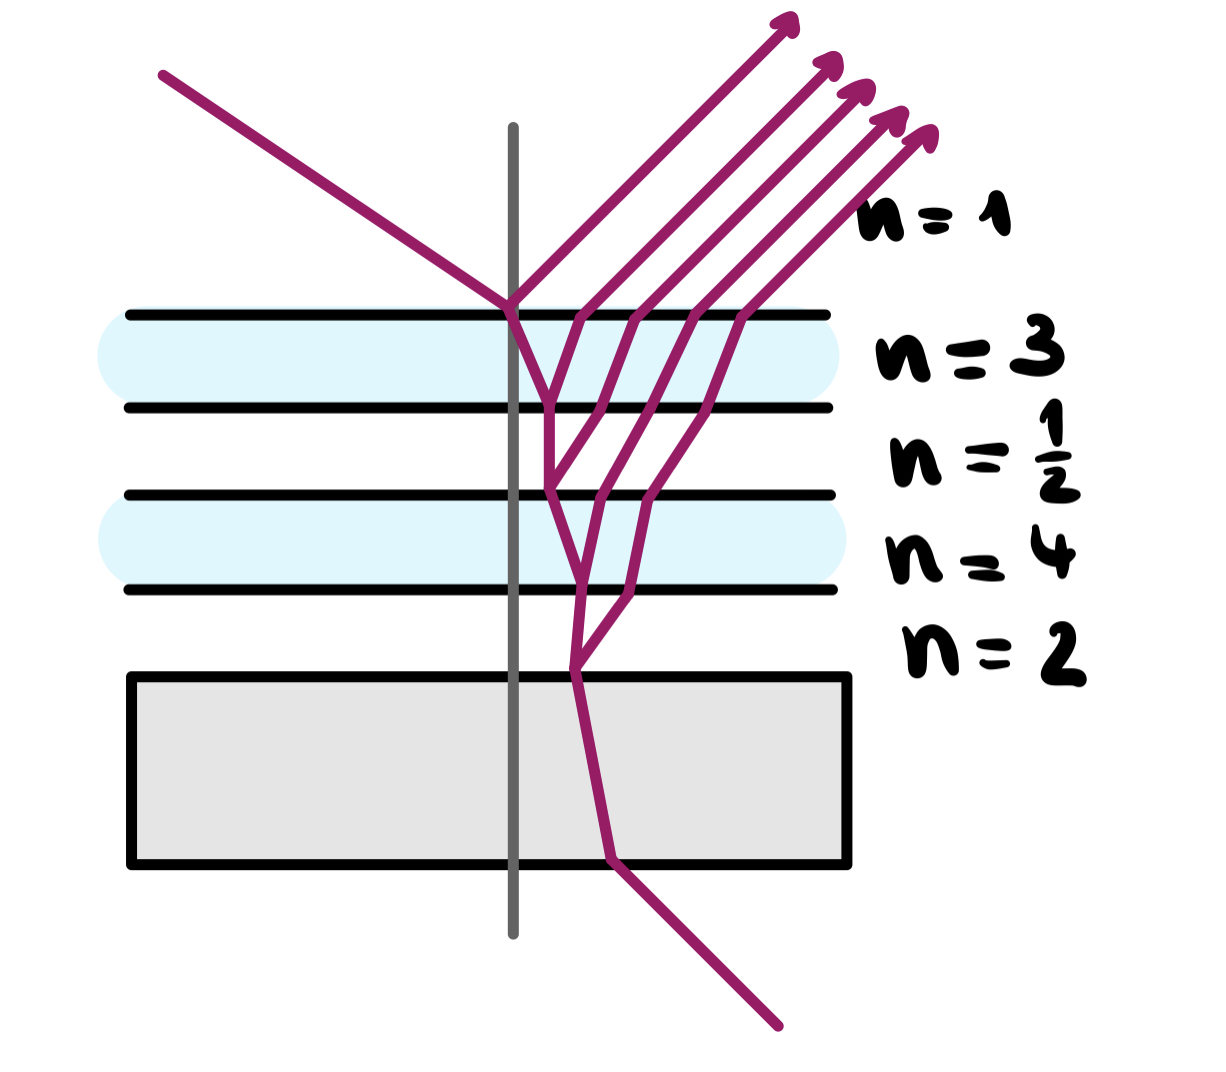
\includegraphics[scale=0.13]{Bilder/FzV/spiegel.jpg}
    \caption{Schematische Darstellung des Strahlengangs in einem Dielektrischen Spiegel mit mehreren Schichten mit verschiedenen Brechungsindizies.}
\end{figure}
